\begin{exercice*}[Graphique cartésien]
    Dans le parc naturel de Genser, il y a beaucoup d'animaux.
    Voici un tableau qui donne le nombre d'individus de quelques espèces.
    
    \smallskip
    $
    \begin{array}{|c|c|c|c|c|}
    \hline
    \text{Animaux} & \text{girafes} & \text{rhinocéros} & \text{guépards} & \text{hyènes}\\
    \hline
    \text{Effectifs} & 32 & 12 & 20 & 16\\
    \hline
    \end{array}
    $
    
    
    \smallskip
    Représenter ces données par un graphique cartésien.   
    
    \hrefMathalea{https://coopmaths.fr/mathalea.html?ex=5S12,s=3,s2=1,s3=4,s4=true&v=l} % On peut personnaliser le texte entre crochets si on veut sinon supprimer les crochets
\end{exercice*}
\begin{corrige}
    %\setcounter{partie}{0} % Pour s'assurer que le compteur de \partie est à zéro dans les corrigés
    %\phantom{rrr}
    Dans le parc naturel de Genser, il y a beaucoup d'animaux.
    Voici un tableau qui donne le nombre d'individus de quelques espèces.
    
    \smallskip
    $
    \begin{array}{|c|c|c|c|c|}
    \hline
    \text{Animaux} & \text{girafes} & \text{rhinocéros} & \text{guépards} & \text{hyènes}\\
    \hline
    \text{Effectifs} & 32 & 12 & 20 & 16\\
    \hline
    \end{array}
    $   
    
    \smallskip
    Représenter ces données par un graphique cartésien.   
    
    {\red    
        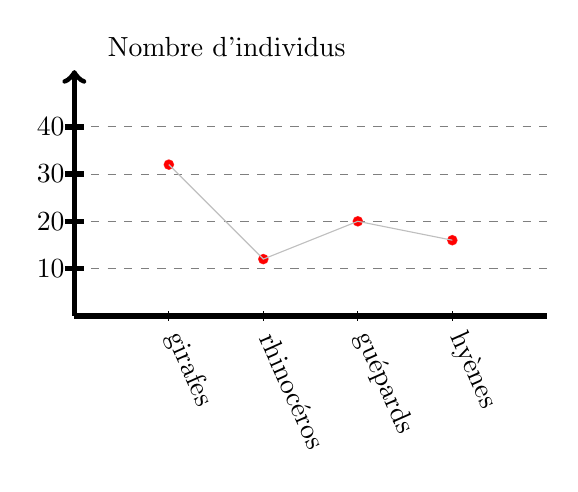
\begin{tikzpicture}[baseline,scale=0.6]
    
        \tikzset{
          point/.style={
            thick,
            draw,
            cross out,
            inner sep=0pt,
            minimum width=5pt,
            minimum height=5pt,
          },
        }        
    
    
        \draw [color={black}] (2,-0.2) node[anchor = west, rotate = -66] {girafes};
        \draw[color ={black}] (2,-0.1)--(2,0.1);
        \draw [color={black}] (4,-0.2) node[anchor = west, rotate = -66] {rhinocéros};
        \draw[color ={black}] (4,-0.1)--(4,0.1);
        \draw [color={black}] (6,-0.2) node[anchor = west, rotate = -66] {guépards};
        \draw[color ={black}] (6,-0.1)--(6,0.1);
        \draw [color={black}] (8,-0.2) node[anchor = west, rotate = -66] {hyènes};
        \draw[color ={black}] (8,-0.1)--(8,0.1);
        
        \draw[color ={black},line width = 2] (0,0)--(10,0);
        \draw[color ={black},line width = 2,->] (0,0)--(0,5.2);
        \draw[color ={black},opacity = 0.5, dashed ] (0,1)--(10,1);
        \draw[color ={black},opacity = 0.5, dashed ] (0,2)--(10,2);
        \draw[color ={black},opacity = 0.5, dashed ] (0,3)--(10,3);
        \draw[color ={black},opacity = 0.5, dashed ] (0,4)--(10,4);
        \draw[color ={black},line width = 2] (-0.2,1)--(0.2,1);
        \draw[color ={black},line width = 2] (-0.2,2)--(0.2,2);
        \draw[color ={black},line width = 2] (-0.2,3)--(0.2,3);
        \draw[color ={black},line width = 2] (-0.2,4)--(0.2,4);
        \draw [color={black},fill opacity = 1] (-0.5,1) node[anchor = center,scale=1] {$10$};
        \draw [color={black},fill opacity = 1] (-0.5,2) node[anchor = center,scale=1] {$20$};
        \draw [color={black},fill opacity = 1] (-0.5,3) node[anchor = center,scale=1] {$30$};
        \draw [color={black},fill opacity = 1] (-0.5,4) node[anchor = center,scale=1] {$40$};
        \draw [color={black},fill opacity = 1] (0.5,5.7) node[anchor = west,scale=1] {Nombre d'individus};
        
        
        \draw[color={{red}},opacity = 0.8,fill opacity = 0.4,preaction={fill,color = red}] (2,3.2) circle (0.1);
        
        \draw[color={{red}},opacity = 0.8,fill opacity = 0.4,preaction={fill,color = red}] (4,1.2000000000000002) circle (0.1);
        
        \draw[color={{red}},opacity = 0.8,fill opacity = 0.4,preaction={fill,color = red}] (6,2) circle (0.1);
        
        \draw[color={{red}},opacity = 0.8,fill opacity = 0.4,preaction={fill,color = red}] (8,1.6) circle (0.1);
        \draw[color={lightgray}] (2,3.2)--(4,1.2000000000000002)--(6,2)--(8,1.6);
    
    \end{tikzpicture}
    }
\end{corrige}

